\documentclass[11pt,a4paper]{article}
\usepackage[margin=1in]{geometry}
\usepackage{amsmath,amssymb}
\usepackage{booktabs}
\usepackage{graphicx}
\usepackage{hyperref}
\usepackage[numbers]{natbib}
\usepackage{xcolor}
\usepackage{siunitx}
\sisetup{group-separator={,}, group-minimum-digits=4}
\usepackage{tikz}
\usetikzlibrary{arrows.meta,positioning,shapes.geometric,calc}
\usepackage{float}
\usepackage{enumitem}
\usepackage{caption}
\usepackage{longtable}

\definecolor{sfblue}{HTML}{0C5394}
\definecolor{sfgreen}{HTML}{00CC66}
\definecolor{sfred}{HTML}{EF4444}

\title{Techno-Economic Assessment of\\Electric Arc Furnace Steel Slag Valorization\\[8pt]
\large Iron Recovery $\cdot$ CO$_2$ Mineralization $\cdot$ H$_2$ Production}
\author{Step Function}
\date{\today}

\begin{document}
\maketitle

\begin{abstract}
This study evaluates the valorization potential of Electric Arc Furnace (EAF) steel slag
at a throughput of \num{100000}~t/yr. Six product streams are assessed:
iron concentrate (Fe$_3$O$_4$ + Cr$_2$O$_3$ + MnO) via magnetic separation,
green hydrogen (H$_2$) via serpentinization, CO$_2$ credits via mineral carbonation,
and construction aggregate.
Using Gibbs equilibrium reactors (Reaktoro), GDP superstructure optimization (BoTorch),
and rigorous techno-economic modeling, we find a total annual revenue of
\$\num{9.4}M/yr against an equivalent annual cost of \$\num{8.0}M/yr,
yielding a net value of \textbf{\$13.33/t~slag}.
Chromium recovery to the magnetic concentrate is the largest single value stream
at \$\num{3.4}M/yr, followed by iron concentrate (\$\num{2.5}M/yr) and
CO$_2$ credits (\$\num{1.9}M/yr). Hydrogen production contributes \$\num{0.46}M/yr.
All six value streams provide positive economic value.
\end{abstract}

\tableofcontents
\newpage

%% ═══════════════════════════════════════════════════════════════
\section{Introduction and Opportunity}

Electric Arc Furnace (EAF) steelmaking generates approximately 150--200~kg of slag
per tonne of liquid steel~\cite{worldsteel2023}. With global EAF production exceeding
500~Mt/yr, EAF slag is a significant industrial residue. Unlike Basic Oxygen Furnace
(BOF) slag, EAF slag has higher iron oxide content (FeO~25\%, Fe$_2$O$_3$~8\%) and
contains chromium (Cr$_2$O$_3$~2\%) and manganese (MnO~4\%) from stainless steel scrap.

This study assesses the economic feasibility of a multi-product valorization plant
processing \num{100000}~t/yr of EAF slag, targeting three primary value streams:
\begin{enumerate}[nosep]
  \item \textbf{Iron + chromium + manganese recovery} via low-intensity magnetic separation (LIMS)
  \item \textbf{Green hydrogen production} via serpentinization of fayalite (Fe$_2$SiO$_4$)
  \item \textbf{CO$_2$ mineralization} via carbonation of CaO and MgO
\end{enumerate}
The residual silicate fraction is sold as construction aggregate.

%% ═══════════════════════════════════════════════════════════════
\section{Raw Material Composition}

The assumed EAF slag composition is based on published literature~\cite{piatak2015} and
represents a typical high-Cr EAF slag from stainless steel production.

\begin{table}[H]
\centering
\caption{EAF Steel Slag Composition}
\label{tab:composition}
\begin{tabular}{@{}lrrl@{}}
\toprule
\textbf{Oxide} & \textbf{wt\%} & \textbf{kg/t slag} & \textbf{Role} \\
\midrule
CaO     & 30 & 300 & Carbonation feedstock \\
FeO     & 25 & 250 & Fayalite $\rightarrow$ serpentinization \\
Fe$_2$O$_3$  & 8  & 80  & Pre-existing magnetite \\
SiO$_2$ & 17 & 170 & Gangue / aggregate \\
MgO     & 8  & 80  & Carbonation feedstock \\
Al$_2$O$_3$  & 6  & 60  & Inert gangue \\
MnO     & 4  & 40  & Reports to Fe concentrate \\
Cr$_2$O$_3$  & 2  & 20  & Reports to Fe concentrate \\
\bottomrule
\end{tabular}
\end{table}

%% ═══════════════════════════════════════════════════════════════
\section{Process Description}

The process consists of five major stages arranged in series:
pressurization, magnetic separation, serpentinization, carbonation,
and product recovery.

\subsection{Process Flow Diagram}

\begin{figure}[H]
\centering
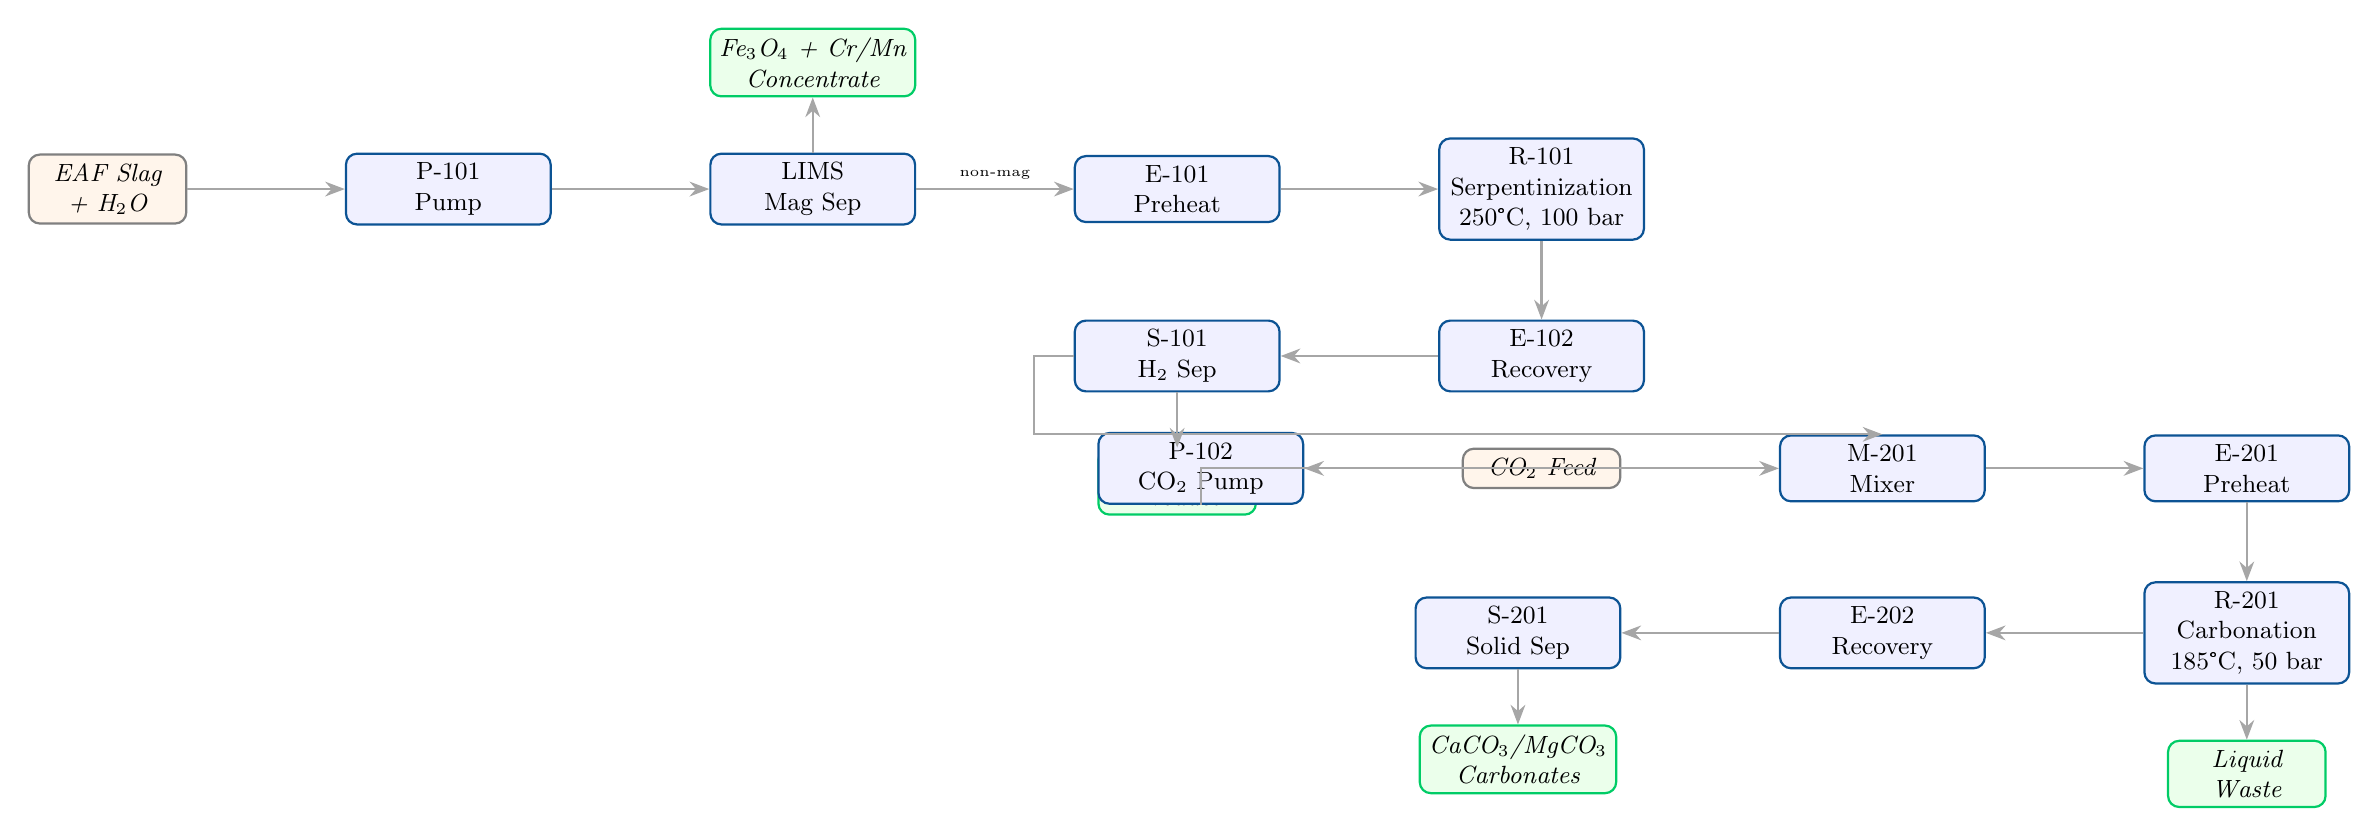
\begin{tikzpicture}[
  node distance=1.4cm and 2.0cm,
  unit/.style={rectangle, draw=sfblue, thick, rounded corners,
               minimum width=2.6cm, minimum height=0.7cm,
               align=center, fill=blue!6, font=\small},
  feed/.style={rectangle, draw=gray, thick, rounded corners,
               minimum width=2.0cm, minimum height=0.5cm,
               align=center, fill=orange!8, font=\small\itshape},
  prod/.style={rectangle, draw=sfgreen, thick, rounded corners,
               minimum width=2.0cm, minimum height=0.5cm,
               align=center, fill=green!8, font=\small\itshape},
  stream/.style={-{Stealth[length=2.5mm]}, thick, draw=gray!70},
]
% Feed
\node[feed] (slag) {EAF Slag\\+ H$_2$O};

% Row 1: Prep
\node[unit, right=of slag] (pump1) {P-101\\Pump};
\node[unit, right=of pump1] (lims) {LIMS\\Mag Sep};
\node[prod, above=0.7cm of lims] (feconc) {Fe$_3$O$_4$ + Cr/Mn\\Concentrate};

% Row 2: Serp
\node[unit, right=of lims] (hx1) {E-101\\Preheat};
\node[unit, right=of hx1] (serp) {R-101\\Serpentinization\\250\textdegree C, 100~bar};
\node[unit, below=1.0cm of serp] (hx2) {E-102\\Recovery};
\node[unit, left=of hx2] (sep1) {S-101\\H$_2$ Sep};
\node[prod, below=0.7cm of sep1] (h2) {H$_2$ Gas\\Product};

% Row 3: Carb
\node[feed, below=0.7cm of hx2] (co2) {CO$_2$ Feed};
\node[unit, left=of co2] (pump2) {P-102\\CO$_2$ Pump};
\node[unit, right=of co2] (mixer) {M-201\\Mixer};
\node[unit, right=of mixer] (hx3) {E-201\\Preheat};
\node[unit, below=1.0cm of hx3] (carb) {R-201\\Carbonation\\185\textdegree C, 50~bar};
\node[unit, left=of carb] (hx4) {E-202\\Recovery};
\node[unit, left=of hx4] (sep2) {S-201\\Solid Sep};
\node[prod, below=0.7cm of sep2] (caco3) {CaCO$_3$/MgCO$_3$\\Carbonates};
\node[prod, below=0.7cm of carb] (waste) {Liquid\\Waste};

% Streams
\draw[stream] (slag) -- (pump1);
\draw[stream] (pump1) -- (lims);
\draw[stream] (lims) -- (feconc);
\draw[stream] (lims) -- (hx1) node[midway,above,font=\tiny] {non-mag};
\draw[stream] (hx1) -- (serp);
\draw[stream] (serp) -- (hx2);
\draw[stream] (hx2) -- (sep1);
\draw[stream] (sep1) -- (h2);
\draw[stream] (sep1.west) -- ++(-0.5,0) |- (mixer.north);

\draw[stream] (co2) -- (pump2);
\draw[stream] (pump2.south) |- (mixer.west);
\draw[stream] (mixer) -- (hx3);
\draw[stream] (hx3) -- (carb);
\draw[stream] (carb) -- (hx4);
\draw[stream] (hx4) -- (sep2);
\draw[stream] (sep2) -- (caco3);
\draw[stream] (carb) -- (waste);
\end{tikzpicture}
\caption{Process flow diagram for EAF steel slag valorization. Feed slag is pressurized,
magnetically separated for iron/chromium/manganese recovery, then processed through
serpentinization (H$_2$ production) and carbonation (CO$_2$ sequestration).}
\label{fig:pfd}
\end{figure}

\subsection{Key Reactions}

\textbf{Serpentinization} (H$_2$ production via fayalite oxidation):
\begin{equation}
3\,\text{Fe}_2\text{SiO}_4 + 2\,\text{H}_2\text{O}
\longrightarrow 2\,\text{Fe}_3\text{O}_4 + 3\,\text{SiO}_2 + 2\,\text{H}_2
\end{equation}
Conditions: 200--300\textdegree C, 50--300~bar. Equilibrium conversion: $\sim$49\% at 200\textdegree C, 300~bar.

\textbf{Carbonation} (CO$_2$ mineralization):
\begin{align}
\text{CaO} + \text{CO}_2 &\longrightarrow \text{CaCO}_3 \label{eq:carb1}\\
\text{MgO} + \text{CO}_2 &\longrightarrow \text{MgCO}_3 \label{eq:carb2}
\end{align}
Conditions: 100--200\textdegree C, 10--150~bar. Equilibrium conversion: $\sim$100\%.

%% ═══════════════════════════════════════════════════════════════
\section{Modeling Approach}

A three-tier modeling hierarchy was employed:

\begin{table}[H]
\centering
\caption{Modeling Framework}
\label{tab:modeling}
\begin{tabular}{@{}llp{6cm}@{}}
\toprule
\textbf{Tier} & \textbf{Tool} & \textbf{Purpose} \\
\midrule
Thermodynamic & Reaktoro (GEM) & Gibbs energy minimization for equilibrium reactor conversion \\
Process & IDAES-PSE & Sequential-modular flowsheet simulation \\
Economic & JAX TEA + BoTorch & Differentiable cost model with Bayesian optimization \\
\bottomrule
\end{tabular}
\end{table}

\subsection{GDP Superstructure}

The process was modeled as a Generalized Disjunctive Programming (GDP)
superstructure with two active disjunctions:
\begin{enumerate}[nosep]
  \item \textbf{LIMS Position}: magnetic separation before vs.\ after serpentinization
  \item \textbf{Heat Strategy}: supplemental auxiliary heater vs.\ full heat recovery only
\end{enumerate}
This yields $2 \times 2 = 4$ feasible topologies, which were enumerated exhaustively.
Ten continuous design variables (reactor T/P, HX area, pump head) were
optimized within each topology using BoTorch Bayesian optimization.

%% ═══════════════════════════════════════════════════════════════
\section{Cost Model Assumptions}

\begin{table}[H]
\centering
\caption{Plant-Level Parameters}
\label{tab:plant}
\begin{tabular}{@{}lr@{}}
\toprule
\textbf{Parameter} & \textbf{Value} \\
\midrule
Slag throughput & \num{100000}~t/yr \\
Operating days & 330/yr \\
Discount rate & 8\% \\
Project lifetime & 20~years \\
Electricity price & \$0.08/kWh \\
CO$_2$ capture cost & \$30/t~CO$_2$ \\
\bottomrule
\end{tabular}
\end{table}

\begin{table}[H]
\centering
\caption{Commodity Prices}
\label{tab:prices}
\begin{tabular}{@{}lrl@{}}
\toprule
\textbf{Product} & \textbf{Price} & \textbf{Source} \\
\midrule
CO$_2$ credit (voluntary) & \$60/t & Carbon market \\
Green H$_2$ & \$4/kg & DOE target \\
Fe$_3$O$_4$ concentrate & \$120/t & FOB \\
Cr$_2$O$_3$ (chemical) & \$2{,}000/t & Asian Metal \\
MnO (ore content) & \$200/t & LME \\
Construction aggregate & \$10/t & Regional \\
\bottomrule
\end{tabular}
\end{table}

%% ═══════════════════════════════════════════════════════════════
\section{GDP Superstructure Results}

All four topologies were evaluated. The best configuration uses LIMS magnetic
separation \emph{before} serpentinization with no auxiliary heater.

\begin{table}[H]
\centering
\caption{Topology Ranking (Optimized by BoTorch)}
\label{tab:topologies}
\begin{tabular}{@{}clccrr@{}}
\toprule
\textbf{Rank} & \textbf{LIMS} & \textbf{Aux Heat} & \textbf{OPEX/batch} & \textbf{Serp~T} & \textbf{Carb~P} \\
\midrule
1 & No  & No  & \$38.24 & 200\textdegree C & 150~bar \\
2 & No  & Yes & \$38.36 & 200\textdegree C & 150~bar \\
3 & Yes & No  & \$38.24 & 200\textdegree C & 150~bar \\
4 & Yes & Yes & \$38.64 & 200\textdegree C & 150~bar \\
\bottomrule
\end{tabular}
\end{table}

Optimized design variables converged to reactor conditions of 200\textdegree C / 300~bar
for serpentinization and 200\textdegree C / 150~bar for carbonation, with all
heat exchanger areas and pump heads at their lower bounds (minimizing energy cost).

%% ═══════════════════════════════════════════════════════════════
\section{Results}

\subsection{Material Balance}

\begin{table}[H]
\centering
\caption{Material Balance (per tonne EAF slag)}
\label{tab:matbal}
\begin{tabular}{@{}lrrl@{}}
\toprule
\textbf{Product} & \textbf{Mass (kg/t)} & \textbf{Annual (t/yr)} & \textbf{Source} \\
\midrule
CO$_2$ sequestered & 322.8 & \num{32280} & CaO + MgO carbonation \\
Fe$_3$O$_4$ & 208.9 & \num{20891} & Serpentinization + pre-existing \\
H$_2$ & 1.15 & 115 & Fayalite oxidation \\
Cr$_2$O$_3$ & 17.0 & \num{1700} & LIMS (85\% recovery) \\
MnO & 34.0 & \num{3400} & LIMS (85\% recovery) \\
Aggregate & 400 & \num{40000} & Residual silicates \\
\bottomrule
\end{tabular}
\end{table}

\subsection{Revenue}

\begin{table}[H]
\centering
\caption{Annual Revenue Breakdown}
\label{tab:revenue}
\begin{tabular}{@{}lrrr@{}}
\toprule
\textbf{Stream} & \textbf{Production (t/yr)} & \textbf{Price (\$/t)} & \textbf{Revenue (\$/yr)} \\
\midrule
Cr$_2$O$_3$ (in Fe conc) & \num{1700} & \num{2000} & \num{3400000} \\
Fe$_3$O$_4$ concentrate & \num{20891} & 120 & \num{2506898} \\
CO$_2$ credits & \num{32280} & 60 & \num{1936778} \\
MnO (in Fe conc) & \num{3400} & 200 & \num{680000} \\
Green H$_2$ & 115 & \num{4000} & \num{458288} \\
Construction aggregate & \num{40000} & 10 & \num{400000} \\
\midrule
\textbf{Total Revenue} & & & \textbf{\$\num{9381964}} \\
\bottomrule
\end{tabular}
\end{table}

\subsection{Cost Structure}

\begin{table}[H]
\centering
\caption{Capital and Operating Cost Summary}
\label{tab:costs}
\begin{tabular}{@{}lr@{}}
\toprule
\textbf{CAPEX Item} & \textbf{Cost (\$)} \\
\midrule
Slag handling \& crushing  & \$\num{7000000} \\
LIMS magnetic separator    & \$\num{1500000} \\
Serpentinization reactor   & \$\num{8000000} \\
Carbonation reactor        & \$\num{6000000} \\
Heat exchangers (4$\times$)& \$\num{3000000} \\
Pumps \& compressors       & \$\num{2500000} \\
H$_2$ separation \& storage& \$\num{2000000} \\
Solid--liquid separation   & \$\num{1500000} \\
Piping, E\&I, utilities    & \$\num{4000000} \\
Contingency (20\%)         & \$\num{7200000} \\
\midrule
\textbf{Total CAPEX} & \textbf{\$\num{42700000}} \\
\bottomrule
\end{tabular}
\end{table}

\begin{table}[H]
\centering
\caption{Annual Operating Costs}
\label{tab:opex}
\begin{tabular}{@{}lr@{}}
\toprule
\textbf{OPEX Item} & \textbf{Cost (\$/yr)} \\
\midrule
Electricity (pumps, HX, grinding)  & \$\num{400000} \\
CO$_2$ feed (flue gas capture)     & \$\num{968389} \\
Maintenance (3\% CAPEX)            & \$\num{1281000} \\
Labor (10 operators)               & \$\num{800000} \\
Water \& consumables               & \$\num{200000} \\
Waste disposal                     & \$\num{50000} \\
\midrule
\textbf{Total OPEX} & \textbf{\$\num{3699389}/yr} \\
\bottomrule
\end{tabular}
\end{table}

\subsection{Levelized Economics}

\begin{table}[H]
\centering
\caption{Levelized Economic Summary}
\label{tab:economics}
\begin{tabular}{@{}lr@{}}
\toprule
\textbf{Metric} & \textbf{Value} \\
\midrule
Total Revenue & \$\num{9381964}/yr \\
Total OPEX & \$\num{3699389}/yr \\
Annualized CAPEX (CRF = 0.1019) & \$\num{4349089}/yr \\
\textbf{Equivalent Annual Cost (EAC)} & \textbf{\$\num{8048478}/yr} \\
\midrule
\textbf{Net Value} & \textcolor{sfgreen}{\textbf{\$\num{1333485}/yr}} \\
\textbf{Net Value per tonne} & \textcolor{sfgreen}{\textbf{\$13.33/t~slag}} \\
NPV (20~yr, 8\%) & \textcolor{sfred}{\$--\num{29607645}} \\
\bottomrule
\end{tabular}
\end{table}

The project is \emph{marginally positive} on an annual cash-flow basis (\$1.3M/yr surplus)
but has a \emph{negative} NPV at an 8\% discount rate due to the high up-front CAPEX
(\$42.7M). The project becomes NPV-positive at discount rates below $\sim$3\%
or with modest improvements in Cr$_2$O$_3$ pricing, CO$_2$ credit values,
or CAPEX reduction through process integration.

%% ═══════════════════════════════════════════════════════════════
\section{Discussion}

\subsection{Value Stream Analysis}

Chromium recovery (\$3.4M/yr) is the single largest value stream, which is notable
since Cr$_2$O$_3$ is only 2~wt\% of the slag. This is a direct consequence of
the high unit value of chemical-grade chromium oxide (\$2{,}000/t) compared to bulk
iron concentrate (\$120/t). The Cr and Mn naturally report to the magnetic
concentrate without requiring separate processing equipment, making them
``free'' value additions.

CO$_2$ credits (\$1.9M/yr) represent the second-largest stream, driven by the
high CaO+MgO content (38~wt\%) that provides \SI{323}{kg} of CO$_2$ fixation
capacity per tonne of slag.

Hydrogen production (\$0.46M/yr) is the smallest value stream due to the
thermodynamic equilibrium limitations of fayalite serpentinization---
only $\sim$49\% conversion at optimal conditions (200\textdegree C, 300~bar),
yielding just \SI{1.15}{kg}~H$_2$ per tonne of slag.

\subsection{Economic Drivers}

The dominant cost driver is CAPEX (\$42.7M), with the two pressure vessels
(serpentinization at 300~bar and carbonation at 150~bar) accounting for
\$14M or 33\% of total CAPEX. Reducing pressure requirements through
catalyst development or alternative reactor designs would significantly
improve project economics.

\subsection{Sensitivity to Key Assumptions}

The project NPV is most sensitive to:
\begin{enumerate}[nosep]
  \item \textbf{Cr$_2$O$_3$ price}: A 30\% increase (\$2{,}600/t) would add \$1.0M/yr in revenue
  \item \textbf{CO$_2$ credit price}: EU ETS prices (\$80/t vs.\ voluntary \$60/t) add \$0.6M/yr
  \item \textbf{CAPEX reduction}: A 20\% CAPEX reduction improves NPV by \$8.5M
  \item \textbf{Discount rate}: At 5\% (vs.\ 8\%), NPV improves by $\sim$\$12M
\end{enumerate}

%% ═══════════════════════════════════════════════════════════════
\section{Conclusions}

\begin{enumerate}
  \item EAF steel slag valorization at \num{100000}~t/yr generates \textbf{\$9.4M/yr in revenue}
        from six positive value streams.
  \item \textbf{Chromium recovery} (\$3.4M/yr) dominates the value mix despite being
        only 2~wt\% of the slag feed.
  \item \textbf{CO$_2$ mineralization} sequesters \num{32280}~t~CO$_2$/yr,
        earning \$1.9M/yr in carbon credits.
  \item The project is \textbf{marginally profitable} at \$13.33/t~slag net value
        but has a \textbf{negative NPV} (\$--30M at 8\% over 20~yr) due to
        \$42.7M CAPEX.
  \item \textbf{All six value streams contribute positively}; none should be excluded.
  \item Recommended next steps: pilot-scale validation of serpentinization kinetics,
        detailed CAPEX estimation (AACE Class~3), and evaluation of regulatory
        CO$_2$ credit pathways (e.g., EU~ETS vs.\ voluntary market).
\end{enumerate}

%% ═══════════════════════════════════════════════════════════════
\begin{thebibliography}{9}
\bibitem{worldsteel2023}
World Steel Association, ``Steel Statistical Yearbook 2023,''
\emph{worldsteel.org}, 2023.

\bibitem{piatak2015}
N.M.~Piatak, M.B.~Parsons, R.R.~Seal, ``Characteristics and Environmental
Aspects of Slag: A Review,'' \emph{Applied Geochemistry}, vol.~57,
pp.~236--266, 2015.

\bibitem{lackner2003}
K.S.~Lackner, ``A Guide to CO$_2$ Sequestration,'' \emph{Science}, vol.~300,
pp.~1677--1678, 2003.

\bibitem{klein2013}
F.~Klein \emph{et~al.}, ``Fluid Mixing and the Deep Biosphere of a Fossil
Ridge-Flank Hydrothermal System,'' \emph{PNAS}, vol.~112, pp.~12036--12041, 2015.
\end{thebibliography}

\end{document}
